%This work is licensed under the Creative Commons 
%Attribution-NonCommercial-ShareAlike 3.0 Unported License. 
%To view a copy of this license, visit 
%http://creativecommons.org/licenses/by-nc-sa/3.0/ 
%or send a letter to Creative Commons, 
%444 Castro Street, Suite 900, Mountain View, 
%California, 94041, USA.

\documentclass[letterpaper,12pt]{report}

\pdfpagewidth 8.5in
\pdfpageheight 11in
\topmargin 0in
\headheight 0in
\headsep 0in
\textheight 8.5in
\textwidth 6in
\oddsidemargin 0.5in
\evensidemargin 0in

% \usepackage[OT1,T1]{fontenc}
\usepackage{caption}
\usepackage{multicol}
\usepackage{epsfig}
\usepackage{afterpage}
\usepackage{graphics}
\usepackage{graphicx}
\usepackage[centertags]{amsmath}
\usepackage{amsfonts}
\usepackage{amsthm}
\usepackage{amsmath}
\usepackage{amssymb}
\usepackage[pdftex]{hyperref}
%\usepackage[spanish]{babel}
% \usepackage{makeidx}

\title{\textbf{Knetledge:} a proposal for optimizing learning strategies 
and knowledge organization}

 \author{\bf \LARGE Pablo Gerardo Padilla 
 Beltr\'an\thanks{\large \bf Planet Earth}\\[0.2in]
 \Large \sffamily pgpb.padilla@gmail.com}

% \date{Avance al 28 de abril de 2008} 
\date{} 

% \makeindex
% \makeglossary
% \parindent 0pt
% \parskip 1ex
% \pagenumbering{roman}
\setlength{\columnsep}{10mm}

% \renewcommand{\baselinestretch}{1.33}
\newcommand{\hi}{\rule{0em}{2.5ex}}
\newcommand{\vi}{\vspace{-.17in}}
\newcommand{\HRule}{\rule{\linewidth}{1mm}}



\begin{document}




% \begin{titlepage}
% %  \setlength{\parindent}{0pt}
% %  \setlength{\parskip}{0pt}
% 
% \begin{center}
%       \begin{tabular}{p{1.3in}p{4.7in}}
%               \begin{flushleft}
%               \includegraphics[width=1in]{image/lines-logo.png}
%               \end{flushleft}
%       &
%               \begin{center}
%               \Large
%               \textbf{INSTITUTO POLIT\'ECNICO NACIONAL}\\[5mm]
%               \normalsize \sffamily
%               \textbf{ESCUELA SUPERIOR DE C\'OMPUTO}\\[1in]
%                                                       
%               \large \sffamily
%               \textbf{Trabajo Terminal n\'umero 2007-088} \\[10mm]
%               ``Una aproximaci\'on al fen\'omeno
%               de Muerte Celular Programada utilizando 
%               t\'ecnicas computacionales'' \\ [15mm]
%               \textbf{Que para obtener el t\'itulo de} \\
%               ``Ingeniero en Sistemas Computacionales con
%               la especialidad en Sistemas''\\[15mm]
%               \textbf{Presenta}\\[5mm]
%               Pablo Gerardo Padilla Beltr\'an\\[0.5in]
%               \textbf{Directores}\\[5mm]
%               M. en C. Rosaura Palma Orozco\hspace{0.2in}
%               Dr. Pablo Padilla Longoria\\
%               \vspace*{10mm}
%               M\'exico D. F.,  Mayo de 2008
%               \end{center}
% %     &
% %             \begin{flushright}
% %             \includegraphics[width=0.9in]{expo-16Nov07/escom.png}
% %             \end{flushright}
%       \end{tabular}
% \end{center}
% \end{titlepage}

\maketitle

% \tableofcontents
% \newpage 
% \listoffigures
% \listoftables 

% \chapter{Some Chapter}

\chapter{Introduction}

\paragraph{How this idea came about}
About July, 2010 I was reading an article titled
``How to write mathematics'' by Paul Halmos\cite{halmos_teach_math}.
More or less at the same time I was watching the series
Into the Universe narrated by Stephen Hawking, plus 
I was very dissapointed with my progress in my personal 
study of mathematics.\par

\indent
It all begun when while I was reading Halmos article
I realized that many of the ideas the article mentioned could
be implemented through a computer program in order 
to save time and effort to math students.\par

\paragraph{Halmos's principles for writting maths}
\indent
Some of the basic ideas from that article are:

\begin{itemize}
 \item Writting self-contained materials
 \item The Spiral plan: iteratively improving the material
 \item Triptic: Say what you're going to say, say it, 
    say what you said.
\item Defined algorithm to determine the order in which
the topics should be presented
\end{itemize}

\indent
The key was to make the process of organizing the topics of 
a given course in a way that they are unobstrusive to the 
student. Thus allowing him to concentrate in the topic at hand.
\par

\paragraph{ Extending the principles to all sciences}

\indent
I have been a fan of science popularizers for about two or three 
years now, and like many of them, I know that ``our future depends
powerfully on how well we understand this Cosmos''.
\par

\subparagraph{Too moral- Change}
\indent
In these times, when people is obsessed with wanting to prescribe
what other people do with information, it is desperating sometimes
that the access to public knowledge be so damn difficult. Non-free Books, 
journals, courses; patents, copyright, and the like limit our capacity
to benefit from the work of others. And then you have to add the 
inherent perceived disorganization of knowledge.
\par

\indent
Although knowledge is very well organized in clumps of 
related concepts, that is generally not the case when it 
comes to non-trivial relations among concepts in what apparently
are separated fields of knowledge.
\par

\subparagraph{ Extending ... continued}
\indent
In order to preserve all the knowledge, we have to actively
preach the importance of it. So by making available to everyone
we should be in better shape.
\par

\indent
Halmos' ideas can be applied analogoustly to other sciences but
not without effort since formal sciences work in quite a different
manner from the natural ones. Mainly in their method of findind 
truths is different, natural sciences are inductive while formal 
sciences are deductive.

\indent
Nevertheless it's worth exploring 
the possibilities of following these general guidelines to attain
a better organization of our current knowledge.
\par

\indent
So, I started writting down a simple design of how could be
achieve this taking advantage of the technology of the day, 
that is, how to have all the knowledge of all the sciences
well-organized, with what for any practical purpose is a centralized
point of access, the Internet.
\par

\paragraph{The basic idea}
\indent
The basic idea is to have a system that allows you to 
find a topic or concept which you want to learn about, you 
provide a profile based on you current knowledge of the
topic and the system is then able to compute the minimal
tree of dependencies, that is, the mininal number of concepts
that are needed for you to learn before you are able to 
actually understand the selected topic or concept.
\par

\paragraph{The ideal case: Maths}

Why are the formal sciences the ideal case? Well it's is because
in mathematics is basically structured in the following manner:
you have a bunch of definitions, a bunch of axioms, and then
you use those two with well defined rules of inference to build
theorems.

\indent
A theorem is a proposition of the form, ''if A, then P´´ where A is one
or many premises and P is a conclusion that follows from A, although
this may not always be obvious.

\indent
There are special kinds of propositions
which have also the form of a theorem, what separates the theorems from 
the other propositions is that a proof for it has been given.
If no proof is given then they are called conjectures, propositions, 
or hypothesis.

\indent
In math, given a proposition the objective is to find a proof for it, to do that
is is possible to use the premises of that proposition and all the 
other definitions, axioms and theorems that have been proved so far.
Of course you won't always need all the premises, axioms and definitions to 
prove a given theorem. In fact in mathematics it's \textbf{always?} 
possible to find a minimal set of premises, axioms and theorems 
to prove a given theorem. 
And that's what makes math the ideal case for a prototype of a network 
of knowledge.

\indent
Given a concept, you can easily trace back the dependencies for it.
In contrast, it is more difficult to organize knowledge in this way
for natural sciences. Definitions change, we have to distinguish 
between causation (A implies B) and correlation (A is linked to B, but 
in a way that we don't understand yet), facts have to be interpreted
in the context of what's known,.... well you get the idea. The 
structure for knowledge in the formal sciences is more static/constant
than the structure for natural sciences, thus easier to organize.


\subsection{About generalizations}
\indent
Throughout the history of maths, and in general of science, 
there have been various instances in which a given set of 
concepts that seemed to be unrelated could later be unified in 
a generalization. This is in part the objective of this
computer system, in a not so ambitious idea, to help us 
identify which concepts seem to have some pattern that suggest
they may be related. This in principle could be done by analyzing
the structure of the network they form.
A more ambitous idea would be to create algorithms to propose
unifications/generalizations of structures that follow a
similar patter in the way they are interconnected.
 
\indent
The hypothesis is that the structure of the interconnectedness between
concepts can tell us something about an underlying principle that could
in principle unify them.


\subsection{About automation}
If it is possible to reliably find patterns in the structure
of knowledge that is in the network, then it may also be
possible to automate the proposal of new theories, automatic
proof of proposed theorems, etc.

\subsubsection{About applications}
\indent
Concepts are also connected with their \textit{applications},
that is, if an abstract concept can be used practically in 
a given scenario then that use is an application of the 
concept. For example, prime numbers have their applications
in the field of cryptography, the theory of evolution has 
repercusions in the design of new drugs, etc.

\indent
We can then also extend the network of concetps to include 
their applications. This way, we can hypothesize that 
analyzing the structure of such relations  concept-application
we may desing algorithms that coudl propose applications for 
given concepts. In principle automatically speeding up the 
proposal of applications.

\subsubsection{Why we need to speed up applications proposals}
\indent
Some believe we're are at an unprecented point of human history
in the sense that science technology had never advanced so fast as it 
is advancing now (which is true in a sense).
I personally believe that this is not enough. I thinks we 
are rather slow in developing new theories and technologies 
that could allow us to get a better understanding of the cosmos.
We have a lot of ideas that we cannot currently implement becasue
nobody has come up with the technology to do it. Some examples 
of this are, interstellar travel, efficient and clean energy 
production, anti-aging technologies, etc.


\indent
By integrating all the current knowledge in a unified computer 
system freely accessible to anyone with internet access, and 
building a social network around science research, advancing 
collaboration instead of competition, publishing publicly new
knowledge, we have a better chance of coming up with a way to 
accelarate the development of our civilization.


\subsubsection{The future of science}
\indent
In the light? of these hypothesis we can envision that 
mathematicians, and scientists in general should find ways 
to delegate research, at least in the traditional sense to 
computer systems, given that it is possible to automate
the research, hypothesys generation, and applications proposal 
process.
 
 \indent
Our efforts should be focused on finding better, and faster 
ways to advance knowlege generation, organization and 
unification.




\subsection{Ojectives}
\begin{itemize}
 \item Minimize the time and effort for learning a 
given concept.
\item Minimize the space needed to store 
information. (Reduce multiplicity)
\item Optimize the organization of knowledge.
\end{itemize}
\chapter{ Motivation }








\subsection{The problem of information}

\noindent
The problem of information can be defined as follows: 
How to store/organize useful information 
(knowledge in the form of information and relations) 
in the best possible way?
\par

\indent
Today when we have a lot of digital information
and we want to organize or at least free some space
in our storage devices, we simply back up everything.
That is exactly the opossite thing to do in order
to solve the problem of information and I will try 
to explain why that is so.
\par


\paragraph*{Exponential growth vs. finite storage}
\indent
We know that the growth of information
can be described better by means of an exponential 
function rather than a linear function. We know
that our ability to fit more data into the same space 
(improve storage technology) has a theoretical limit 
and a technological one.
\par

\indent
So, we have in the one hand, something that grows faster
as time passes, against something that is constant in the limit
( i. e., the theoretical storage limit is a constant).
\begin{Large}\textbf{Is this true?}\end{Large}
\par


\section{Problem: Organization of knowledge}

\indent
The span of recorded history is of about five thousand years
 \cite{wiki:ancient-hist} and we have generated an inmemse 
 output of information.
 
 \paragraph{Multiplicity}
 Different cultures have arrived to the same concepts thus
 creating multiplicity.
 
 
 Multiplicity being, at least in part, a consequence of the 
 inability to publicly share information easily, this in 
 turn due to lack of technology.
 
 \subparagraph{Distributed nature of knowledge}
 It is a common scenario that a student trying to undertand
 a given topic has to resort to dive into the possbible 
different references has have been advised to check. 

Often, he ends up taking different parts from different
references, be it because of the quality of exposition, 
coverage of the topics in the different references, etc.

So, the distributed nature of the way we organize knowledge
today is a burden when we need to connect certain concepts
or when we want to keep different parts of the approach to 
the topic by the different references.

In any case, this is a waste of time, since as long as the
discussed topic is a mature topic (meaning that the theory, 
facts, etc. has been established for a fair amount of time), 
there should be a standar syllabus for addressing it given 
a predefined objetive. Topics can be studied in different 
ways depending on the final objetive, or reason of why the
concept is studied.


 
 \paragraph{The Internet's role in the organization of knowledge}
 Organizing  the information of a country/state/region 
is not an easy task, let alone organizing all the information
in the world. Nevertheless, the advances in comunication 
technologies makes it possible to share information almost
effortlessly through the internet.

\paragraph{Reducing the problem: Organizing knowledge}
This is the time when we can take advantage of the already 
created infrastructure to build upon it a system that 
enable us to organize all the information in the world.

Of course the easiest way to procced in order to do that is
to modularize the problems, so let's start not with the whole
knowledge of the world, let's organize that which we will call
in this document 'knowledge'.

Knowledge is in itself different from  infomation in the sense
that information is any data that we can think of, while knowledge
is pieces of data connected through relashionships. We may have to 
establish our own 'practical' definitions so to not deviate
in philosophical questions on what is data, information, knowledge, 
wisdom and so on.

So, let's agree that knowledge consists of a set of concepts 
which hold a relation among each other, this relation can be
of one of many possible types.

\paragraph{Ideal case: Mathematics}
To simplify even more the approach we will begin with the 
the formal sciences, Mathematics. The reason as to why start
with it can be answered rather easily, but I will elaborate 
on that to make things real clear.

Mathematics concerns itself with definitions, axioms and their 
consequences. You take a bunch of definitions, propose, verb??
some axioms and then use a set of strictly defined rules (operational 
semantics) to derive implications and other types of relations.

Once you derive a consequence, you can call it a theorem, which 
once demonstrated becomes an axiom.

Now, in mathematics it is comparatively easy to decide which axioms, 
definitions and rules are necesary to arrive from one thorem to 
another, that is, we can discard those that are not used in the 
particular derivation of a given theorem.

This fact makes mathematics very suitable for organizing the relationships
among theorems in a network structure in which each node is connected
to other nodes only if they have some relation. Relations 
can be of various types, the fastes to think about is 
dependence, that is, when in order to prove something you 
have to make use of other thing.

\paragraph{Optimizing Organization: discarding unsed premisses}
Again, in maths, it is easy to discard unused premisses which makes it
easy to model the interelashionships among concepts as a network.

In other sciences, it's sometimes not as easy to discard premisses
since the intrinsic structure of them is different from maths.
In fact, the very way in which the formal sciences and the natural
ones advances is quite different.

\paragraph{Formal vs. Natural Sciences}
On the side of the formal sciences, you propose certain definitions, 
then postulate certain axioms and finaly use formal rules to derive 
consequences, and a consequence is said to be true if it can be
derived in a recognizable manner from the definitions and axioms.

In the natural sciences however, the truth of a proposition has
to based on the available evidence of the event that the proposition
is describing. This kind of evidence has downsides. The evidence may
not be conclusive due to different interpretantions of the facts, or 
other factors...



\section{Problem: The exponential function}




\section{Problem: Multiplicity}
\label{multiplicity}
\indent
 When a student begins to learn something, he/she
 depends on the abilities of his tutor to choose the 
 material to study for a given course.
 \par
 
 \indent
 Once he has the basic bibliography, he often finds
 that there is multiplicity in the content of the 
 various references, that is, there are topics that
 are addressed in more than one source.
 \par
 
 \indent
 The student is in a dilemma, he usually doesn't
 have the time to read all the references, but he
 may read the one which may not be the most useful 
 or appropiate to his learning style.
 \par
 
 \indent
 The student is then forced to explore the different
 references in order to find which may be the best 
 path of study.
 \par



\paragraph{Studying: Blind exploration of the topics}

\indent
We may imagine he exploration of the references as 
exploring the different branches of a tree, in which 
the nodes represent the key concepts and the links 
the connecting ideas between those concepts.
\par

\indent
In a typical scenario the student is on his own exploring 
different references and each attempt to undertand a concept
may be regarded as a branch in the tree. Since he has a 
buch of references but doesn't really know them this tree 
has multiple branches leading to the same concept, that 
is multiplicity of branches. 
\par

\indent
That's not always a bad thing, if the branches are legit, that
is, they represents mutually exclusive paths to the same concept.
\par

\indent
Unfortunately more often than not the concepts explained in 
different references are the same and there should be a standarized
way to present them. 
\begin{Large}\textbf{(Why?)}\end{Large}.
\par

\begin{figure}[htp]
 \centering
 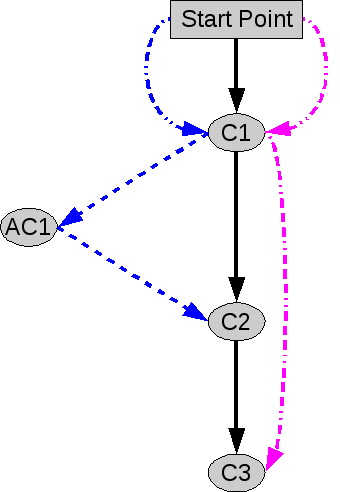
\includegraphics[width=2in]{../img/blind-exploration-tree.png}
 \caption{Blind exploration of ...}
 \label{fig:blind-exploration-tree}
\end{figure}
\section{General solutions - not detailed}
\subsection{Possible Solution}
\indent
Instead of backing up everything, what we need is:

\begin{itemize}
 \item Better ways to organize knowledge
 \item Reduce multiplicity
    \footnote{Check the section \ref{multiplicity}} 
    of knowledge. 
\end{itemize}
\par



\section{Unified access interface}

What this idea proposes is, among other things, the centralized
access to knowledge, given that it is organized in a way that 
multiplicity is reduced and the problems caused by distributed
knowledge are minimized by merging the coverage of topics.

\section{Visual aids: enhancing our ability to relate concepts}

\section{Case Study: Mathematics}

\chapter{Implications}


\subsection{Implications: Space exploration, colinization of exo-planets}

\begin{itemize}
 \item Accelerated learning
 \item Compacted useful knowledge
\end{itemize}


% \input{solutions_detail}
\section{Concepts, relationships and the network}
The whole idea revolves around the idea of concepts, 
their relationships and the network structure 
that arises.

\begin{figure}[ht]
 \begin{center}
    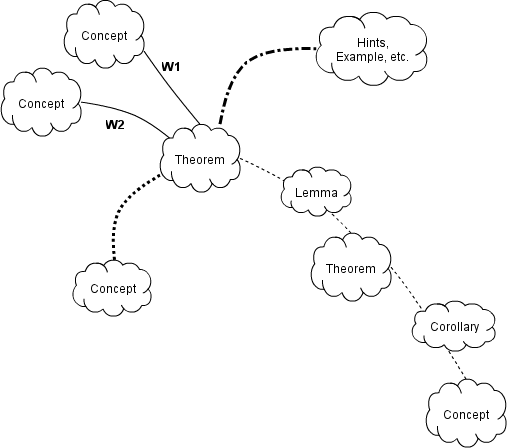
\includegraphics[width=4in]{../img/knet_general.png}
 \end{center}
    \caption{Network of concepts.}
    \label{fig:network_concepts}
\end{figure}



\section{Tech Specs}

\subsection{Social network}
The idea is to build kind of a social network in which
the objective is to advance the understanding and the
organization of math concepts.

\subsection{Re-use not re-invent}
Todays social networks provide most of what would be
needed to implement Knetledge.

Some of the requiered specs are:

\begin{itemize}
 \item Video chat
 \item Voice chat
 \item Shared spaces. Blackboard for brainstorming
 \item Simultaneus edit capabilities
 \item Local copies of subsets of the network
 \item User profile tracking
 \item User profile preferences
 \item Currently working on
 \item Topic: contributors, etc
 
\end{itemize}


\subsection{Graph databases}
There's a lot to learn about Graph databases but it
seems like they would be ideal to implement the kind
of schema that would result from organizing knowledge.

Have to investigate more on the associative data model.
Basically it says that nodes are stored in one table
while relationships between nodes are stored in another 
table which contains information about source and target 
node, and the type of relationships between the connected
nodes.

\subsection{User profile}
\begin{itemize}
 \item Level of Abstraction. This is the level at which 
 the user usually likes to browse concepts.
 \item Areas of interest.
 \item List of known concepts.
 \item Contributions
\end{itemize}

\subsection{Workspace}
A workspace is a set of worksheets, each one containing
a \textbf{board} in which the user can edit a subset of the 
network locally (offline) using a set of tools.

The subset can be then send to a set of experts to 
be reviewed and after that it can be accepted as part of the 
network that is publicly available to everyone.

Of course each person can choose who they share their personal
work with, just like you can set visibility parameter to 
your post on almost any social network.

\section{The Board}
Some of the actions a users can do while in the board are:
\begin{itemize}
 \item Create a new or add an existing concept to the board.
 \item Remove a node
 \item Create a new relationship or add an existing one
 \item Discover relationships. Shows you a list of existing 
relationships so that the user can choose which one are interesing
for the particular aspect s/he is going to work on
\item Save/load the state of the board. Kind of like version control.
The interface should provide tools for easy comparison between different
versions of the board.
 
\end{itemize}


\section{Typical session}
After logging in the user can access the information in the network
by the two most common method, browse and search.

\subsection{Browse}
There should be categories that can be universal or created
by the user, like filter searches

\subsection{Search}
Should include the most common filters:
\begin{itemize}
 \item Topic/related concepts
 \item Contributors
 \item Abstraction levels
 \item Content type: multimedia, text, etc.
\end{itemize}

Other features
\begin{itemize}
 \item Watch later like youtube
 \item Add to board
\end{itemize}



\section{Peer review}

The network should provide the tools for making it easy
to asses the validity of a subset of the network submitted
for revision.

\section{Colaboration}
It should allow simultaneous collaboration in real-time something
similar to what google wave was.



\section{Algorithms}
\begin{itemize}
 \item Find relationships
 \item Propose relationships/applications. This can be used
 to generalize concepts thought to be unrelated
 \item Create new nodes
 \item Automated proof
\end{itemize}


\section{Publishing}
It should provide tools for comparing, merging subsets of the
network in order to facilitate the addition of new concepts
to the network.


% \pagenumbering{arabic}

% 

% %%%%%%%%%%%%%%%%%%%Appendix%%%%%%%%%%
\appendix
\chapter{Definitions and conventions}

\section{From information to Knowledge}
\paragraph{Information}
\indent
We will regard as information anything that can be
represented in some manner.
\par

\indent
The previous definition is very simple, and ambiguous.
But in this case, ambiguous is good since it allows
us to extend the concept to practically everything.
\par

\paragraph{Concept}
\indent
We will use the dictionary defition of the word concept, 
which is: ''a single meaning of a term´´.
\par

\paragraph{Knowledge}
\indent
As a philosophical concept, the definition of knowledge is, and
will probably be under a lot of debate. Nevertheless we can
propose a practical definition for the sake of our pursposes.
Let's call knowledge a composite set, a set of concepts, 
as defined here, and a set of relationships between those concepts.
\par

\indent
We can represent knowledge as a network in which the nodes represent
the concepts related to a given area of knowledge, and the 
links between the nodes as the relationships between interconnected
concepts.
\par


%%%%%%%%%%%%%%%%glossary



%%%%%%%%%%%%%%%%Bibliography%%%%%%%%%%%5

% \phantomsection
% \addcontentsline{toc}{chapter}{Bibliograf\'ia y referencias}

% \def\bibname{Bibliograf\'ia y referencias}
% \bibliographystyle{plain}
% \nocite{}
% 
% \bibliography{references}


% \printindex
\end{document}
